\section{Přechodné jevy druhého řádu}

Uvažujme sériový elektrický obvod na obrázku \ref{fig:druhy_rad_rlc} tvořený rezistorem $R$, induktorem $L$ a kapacitorem $C$ napájený stejnosměrným zdrojem o napětí $U_0$. 
\begin{figure}[h!]
\centering
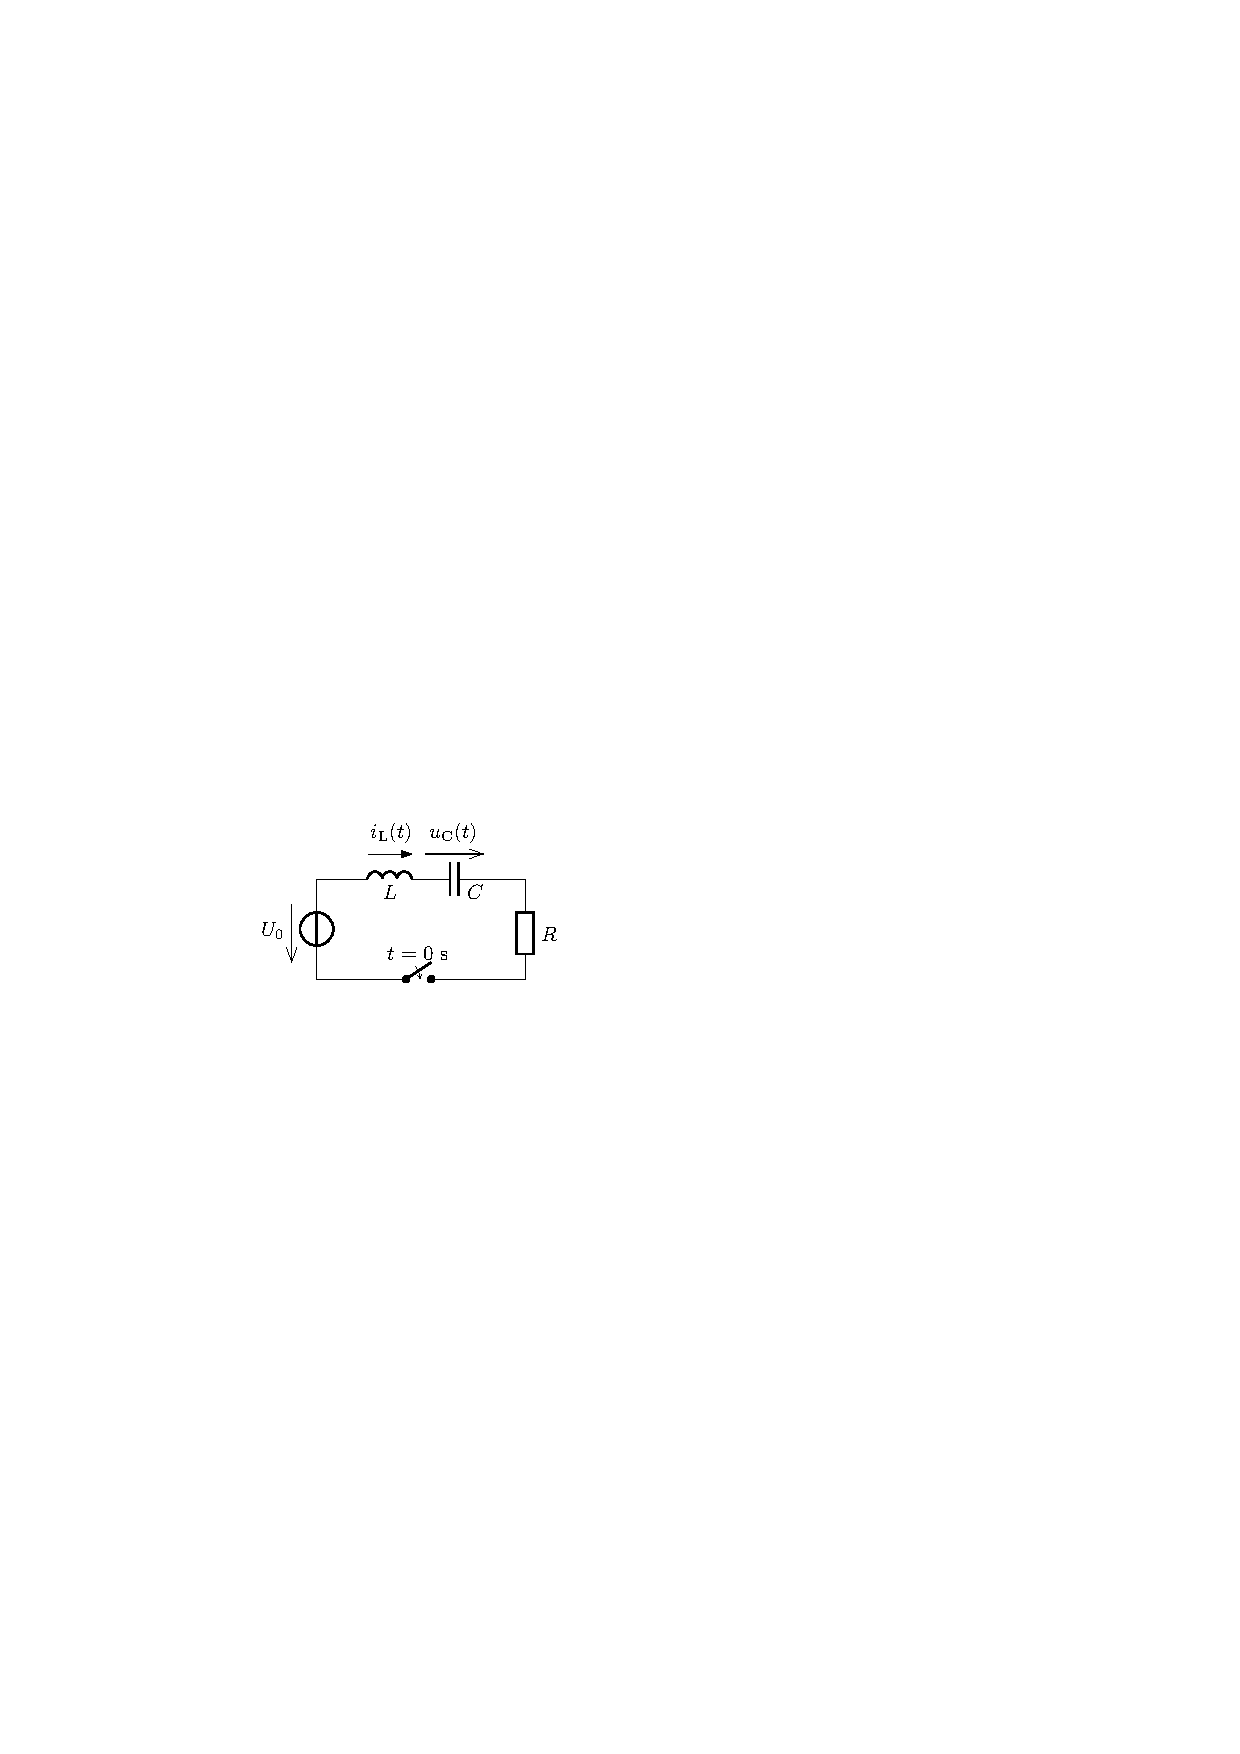
\includegraphics[]{prechodne_jevy/druhy_rad/rlc.pdf}
\caption{Sériová obvod druhého řádu}
\label{fig:druhy_rad_rlc}
\end{figure}
Vyjdeme opět z napěťového Kirchhoffova zákona. Součet napětí na jednotlivých prvcích obvodu je roven napětí zdroje
$$
u_\mathrm{R} + u_\mathrm{L} + u_\mathrm{C} = U_0
$$
Napětí na rezistoru, induktoru a kapacitoru vyjádříme
$$
u_\mathrm{R} = Ri_\mathrm{L} = RC \frac{\dif u_\mathrm{C}}{\dif t},~~~~~
u_\mathrm{L} = L \frac{\dif i_\mathrm{L}}{\dif t} = LC \frac{\dif^2 u_\mathrm{C}}{\dif t^2},~~~~~u_\mathrm{C} = u_\mathrm{C}
$$
Po dosazení získáme diferenciální rovnici pro napětí na kapacitoru $u_\mathrm{C}$ ve tvaru
$$
\frac{\dif^2 u_\mathrm{C}}{\dif t^2} + \frac{R}{L} \cdot \frac{\dif u_\mathrm{C}}{\dif t} + \frac{1}{LC} \cdot u_\mathrm{C} = \frac{U_0}{LC}.
$$
Diferenciální rovnici můžeme ovšem rovněž odvodit pro proud induktorem $i_\mathrm{L}$ s využitím následujících vztahů
$$
u_\mathrm{R} = Ri_\mathrm{L},~~~~~
u_\mathrm{L} = L \frac{\dif i_\mathrm{L}}{\dif t} ,~~~~~u_\mathrm{C} = \frac{1}{C} \int_o^t i_\mathrm{L} \dif t
$$
Získáme
$$
Ri_\mathrm{L} + L \frac{\dif i_\mathrm{L}}{\dif t} + \frac{1}{C} \int_o^t i_\mathrm{L} \dif t = U_0.
$$
Uvedenou rovnici můžeme integrovat a po jednoduché úpravě dostaneme
$$
\frac{\dif^2 i_\mathrm{L}}{\dif t^2} + \frac{R}{L} \cdot \frac{\dif i_\mathrm{L}}{\dif t} + \frac{1}{LC} \cdot i_\mathrm{L} = 0.
$$
Uvažujeme nulové počáteční podmínky. Napětí na kapacitoru bylo na počátku děje nulové
$$
u_\mathrm{C}(0+) = 0.
$$
Proud induktorem byl rovněž nulový
$$
i_\mathrm{L}(0+) = C \frac{\dif u_\mathrm{C}}{\dif t} \left( 0+ \right) = 0
$$
Řešení diferenciální rovnice sestává z obecného $u_o$ a partikulárního řešení $u_p$
$$
u_\mathrm{L} = u_o + u_p.
$$
Nejprve se zaměříme na řešení homogenní rovnice. Charakteristickou rovnici k uvedené diferenciální rovnici (napěťové i proudové) lze zapsat ve tvaru kvadratické rovnice
$$
\lambda^2 + \frac{R}{L} \lambda + \frac{1}{LC} = 0
$$
s kořeny
$$
\lambda_{1,2} = -\frac{R}{2L} \pm \sqrt{\left( \frac{R}{2L} \right)^2 - \frac{1}{LC}}.
$$
S využitím substituce $\beta = \frac{R}{2L}$ a $\omega_0 = \frac{1}{\sqrt{LC}}$ zapíšeme rovnici ve tvaru
$$
\lambda_{1,2} = -\beta \pm \sqrt{\beta^2 - \omega_0^2} = -\beta \pm \alpha,
$$
kde $\omega_0$ je rezonanční frekvenci obvodu a konstantu $\beta$ lze interpretovat jako činitel tlumení. 

Rozeznáváme tři stavy RLC obvodu:
\begin{enumerate*}
\item $\beta > \omega_0$, aperiodický děj,
\item $\beta = \omega_0$, obvod na mezi aperiodicity,
\item $\beta < \omega_0$, kmitavý děj.
\end{enumerate*}
Kritický odpor $R_\mathrm{k}$, při kterém se obvod nachází na mezi aperiodicity, lze vyjádřit z podmínky
$$
\beta = \omega_0~~~ \rightarrow ~~~\left( \frac{R_\mathrm{k}}{2L} \right)^2 = \frac{1}{LC}~~~ \rightarrow ~~~R_\mathrm{k} = 2 \sqrt{\frac{L}{C}}.
$$
Partikulárním řešením je ustálený stav. Kapacitor bude po odeznění přechodného děje nabit na napětí zdroje a obvodem nebude procházet žádný proud 
$$
u_\mathrm{C}(\infty) = U_0,~~~~~~
i_\mathrm{L}(\infty) = 0.
$$

\subsubsection{Aperiodický děj}

V případě kladného diskriminantu ($\beta > \omega_0$) hovoříme o aperiodickém ději. Kořeny charakteristické rovnice $\lambda_{1,2}$ jsou kladná reálná čísla. Řešení diferenciální rovnice předpokládáme ve tvaru součtu dvou exponenciálních funkcí
$$
u_\mathrm{C} = K_1 \cdot \me^{\lambda_1 t} + K_2 \cdot \me^{\lambda_2 t} + U_0.
$$
Časové konstanty lze zapsat ve tvaru
$$
\tau_1 = - \frac{1}{\lambda_1} = \frac{1}{\beta - \alpha},~~~~~
\tau_2 = - \frac{1}{\lambda_2} = \frac{1}{\beta + \alpha},~~~~~
\tau_2 > \tau_1
$$
Pro dosazení počátečních podmínek, je nejprve nutné provést časovou derivaci uvedené rovnice 
$$
\frac{\dif u_\mathrm{C}}{\dif t} = K_1 \lambda_1 \cdot \me^{\lambda_1 t} + K_2 \lambda_2 \cdot \me^{\lambda_2 t}.
$$
Po dosazení počátečních podmínek dostame dvě algebraické rovnice
$$
K_1 + K_2 + U_0 = 0
$$
a
$$
K_1 \lambda_1 + K_2 \lambda_2 = 0
$$
Jejich řešením získáme konstanty $K_1$ a $K_2$. Proud kapacitorem je úměrný časové derivaci napětí
$$
i_\mathrm{L} = i_\mathrm{C} = C \frac{\dif u_\mathrm{C}}{\dif t} = C \left( K_1 \lambda_1 \cdot \me^{\lambda_1 t} + K_2 \lambda_2 \cdot \me^{\lambda_2 t} \right).
$$

\subsubsection{Obvod na mezi aperiodicity}

V případě nulového diskriminantu ($\beta = \omega_0$) hovoříme o ději na mezi aperiodicity. Kořen charakteristické rovnice $\lambda_{1,2}$ je dvojný a je jím kladné reálné číslo $\lambda = - \frac{R}{2L} = - \beta$. Řešení diferenciální rovnice předpokládáme ve tvaru
$$
u_\mathrm{C} = \left( K_1 + K_2 t \right) \me^{\lambda t} + U_0.
$$
Časovou konstantu lze zapsat ve tvaru
$$
\tau = - \frac{1}{\lambda} = \frac{1}{\beta}.
$$
Časová derivace uvedené diferenciální rovnice 
$$
\frac{\dif u_\mathrm{C}}{\dif t} = \left( K_1 \lambda + K_2 \lambda t + K_2 \right) \me^{\lambda t}.
$$
Po aplikaci počátečních podmínek dostame dvě algebraické rovnice
$$
K_1 + U_0 = 0
$$
a
$$
K_1 \lambda + K_2 = 0
$$
Jejich řešením získáme konstanty $K_1$ a $K_2$. Proud kapacitorem je úměrný časové derivaci napětí
$$
i_\mathrm{L} = i_\mathrm{C} = C \frac{\dif u_\mathrm{C}}{\dif t} = C \left( K_1 \lambda + K_2 \lambda t + K_2 \right) \me^{\lambda t} .
$$

\subsubsection{Kmitavý děj}

V případě záporného diskriminantu ($\beta < \omega_0$) hovoříme o kmitavém ději. Kořeny charakteristické rovnice $\lambda_{1,2}$ jsou komplexně sdružená čísla a lze je zapsat ve tvaru
$$
\lambda_{1,2} = - \beta \pm \mj \omega_\mathrm{d},
$$
kde parametr $\omega_\mathrm{d} = \alpha = \sqrt{\beta^2 - \omega_0^2}$ nazýváme frekvence vlastních kmitů. Řešení diferenciální rovnice předpokládáme opět ve tvaru
$$
u_\mathrm{C} = K_1 \cdot \me^{\left( - \beta + \mj \omega_\mathrm{d} \right) t} + K_2 \cdot \me^{\left(- \beta - \mj \omega_\mathrm{d} \right) t} + U_0 = \me^{- \beta t} \left( K_1 \cdot \me^{\mj \omega_\mathrm{d} t} + K_2 \cdot \me^{- \mj \omega_\mathrm{d} t} \right) + U_0.
$$
S využitím Eulerovy identity
$$
\me^{\mj \varphi} = \cos \varphi + \mj \sin \varphi,~~~~~
\me^{- \mj \varphi} = \cos \varphi - \mj \sin \varphi.
$$
dostaneme řešení ve tvaru
$$
u_\mathrm{C} = \me^{- \beta t} \left[ K_1 \left( \cos \omega_\mathrm{d} t + \mj \sin \omega_\mathrm{d} t \right) + K_2 \left( \cos \omega_\mathrm{d} t - \mj \sin \omega_\mathrm{d} t \right) \right] + U_0 =
$$
$$
= \me^{- \beta t} \left[ \left( K_1 + K_2 \right) \cos \omega_\mathrm{d} t + \mj \left( K_1 - K_2 \right) \sin \omega_\mathrm{d} t \right] + U_0.
$$
Z uvedeného vztahu je patrné, že napětí na kapacitoru bude kmitat s periodou $T~=~\frac{2 \pi}{\omega_\mathrm{d}}$ a dále bude exponenciálně tlumené. Konstanty $K_1$ a $K_2$ opět získáme dosazením počátečních podmínek.

Na obrázku \ref{fig:obvod_rlc_napeti} je zobrazen průběh napětí na kapacitoru v případě aperiodického děje, kmitavého děje a děje v obvodu na mezi aperiodicity. Obrázek \ref{fig:obvod_rlc_proud} zobrazuje průběh proudu v obvodu.

\begin{figure}[h!]
\centering
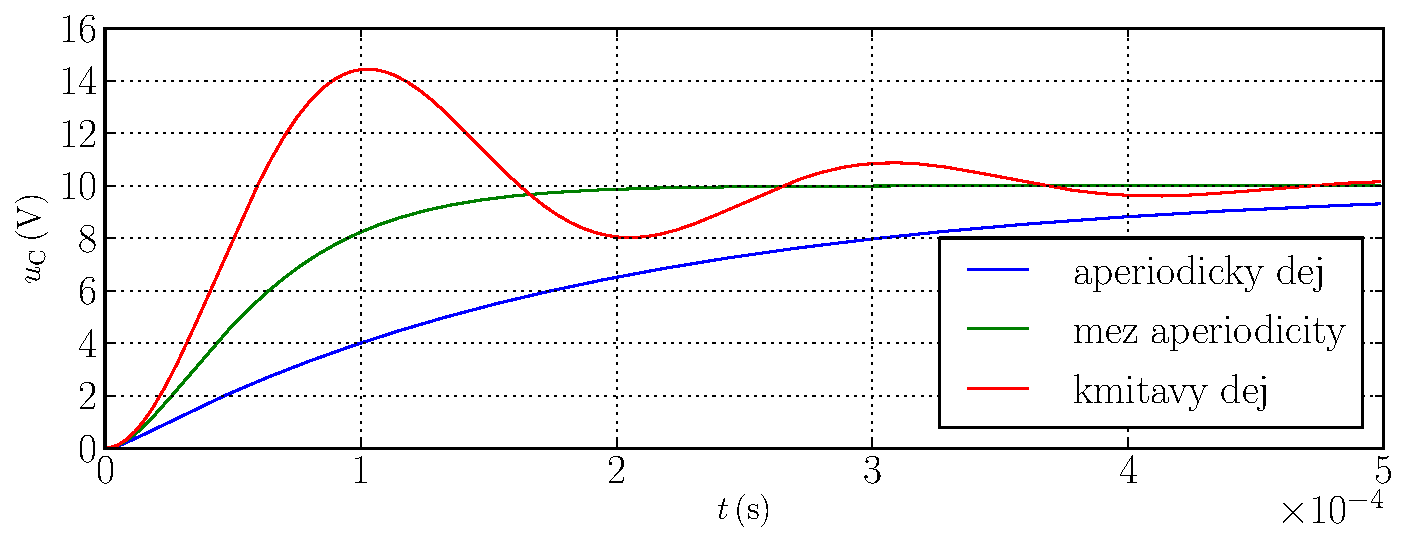
\includegraphics[width=13cm]{prechodne_jevy/druhy_rad/obvod_rlc_napeti.pdf}
\caption{Sériový RLC obvod: napětí na kapacitoru}
\label{fig:obvod_rlc_napeti}
\end{figure}

\begin{figure}[h!]
\centering
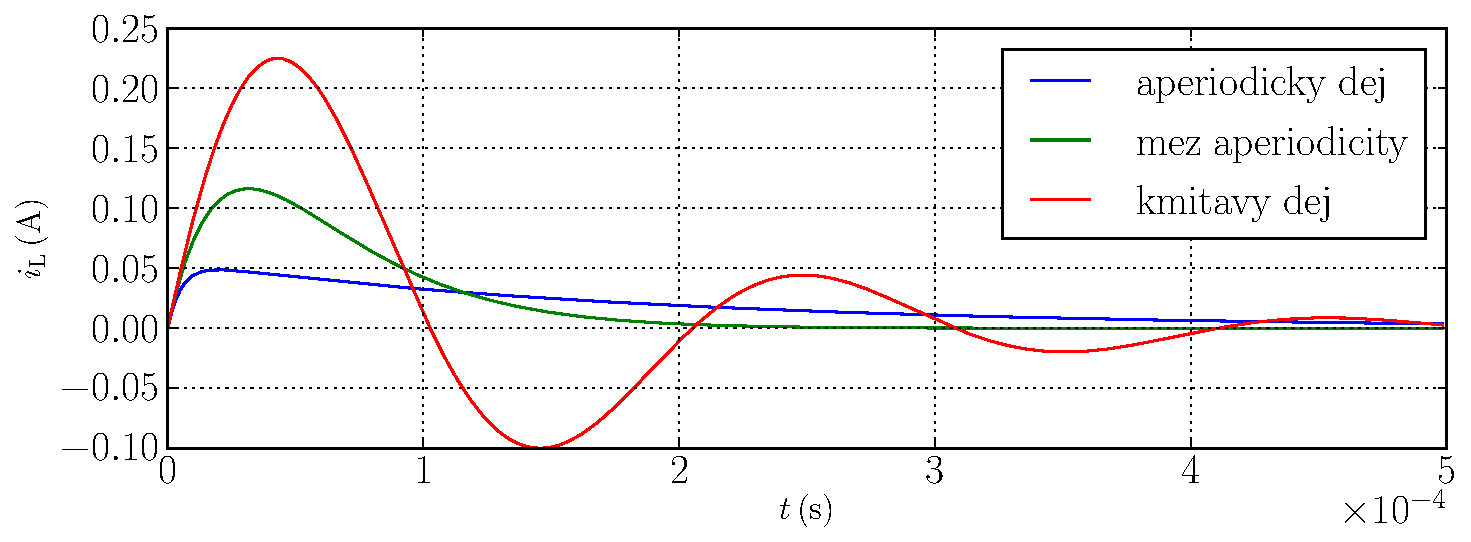
\includegraphics[width=13cm]{prechodne_jevy/druhy_rad/obvod_rlc_proud.pdf}
\caption{Sériový RLC obvod: proud induktorem}
\label{fig:obvod_rlc_proud}
\end{figure}

\subsubsection{Netlumený kmitavý děj}

Speciálním případem kmitavého děje je netlumený kmitavý děj, který nastane při nulovém tlumení obvodu $\beta = 0$. Nutno poznamenat, že tento jev je ideální případ při nulové rezistivitě odporu $R$.

\subsection{Příklady}

Uvažujte obvod dle obrázku \ref{fig:druhy_rad_priklad_1} napájený stejnosměrným zdrojem s napětím $U_0 = 10~\mathrm{V}$ s následujícími parametry: $R_1 = 40~\mathrm{\Omega}$, $R_2 = 40~\mathrm{\Omega}$, $L = 0,4~\mathrm{H}$ a $C = 30~\mathrm{\mu F}$. Vyšetřete průběh proudu $i_\mathrm{L}$ induktorem. Před přechodným dějem se obvod nachází v ustáleném stavu.
\begin{figure}[h!]
\centering
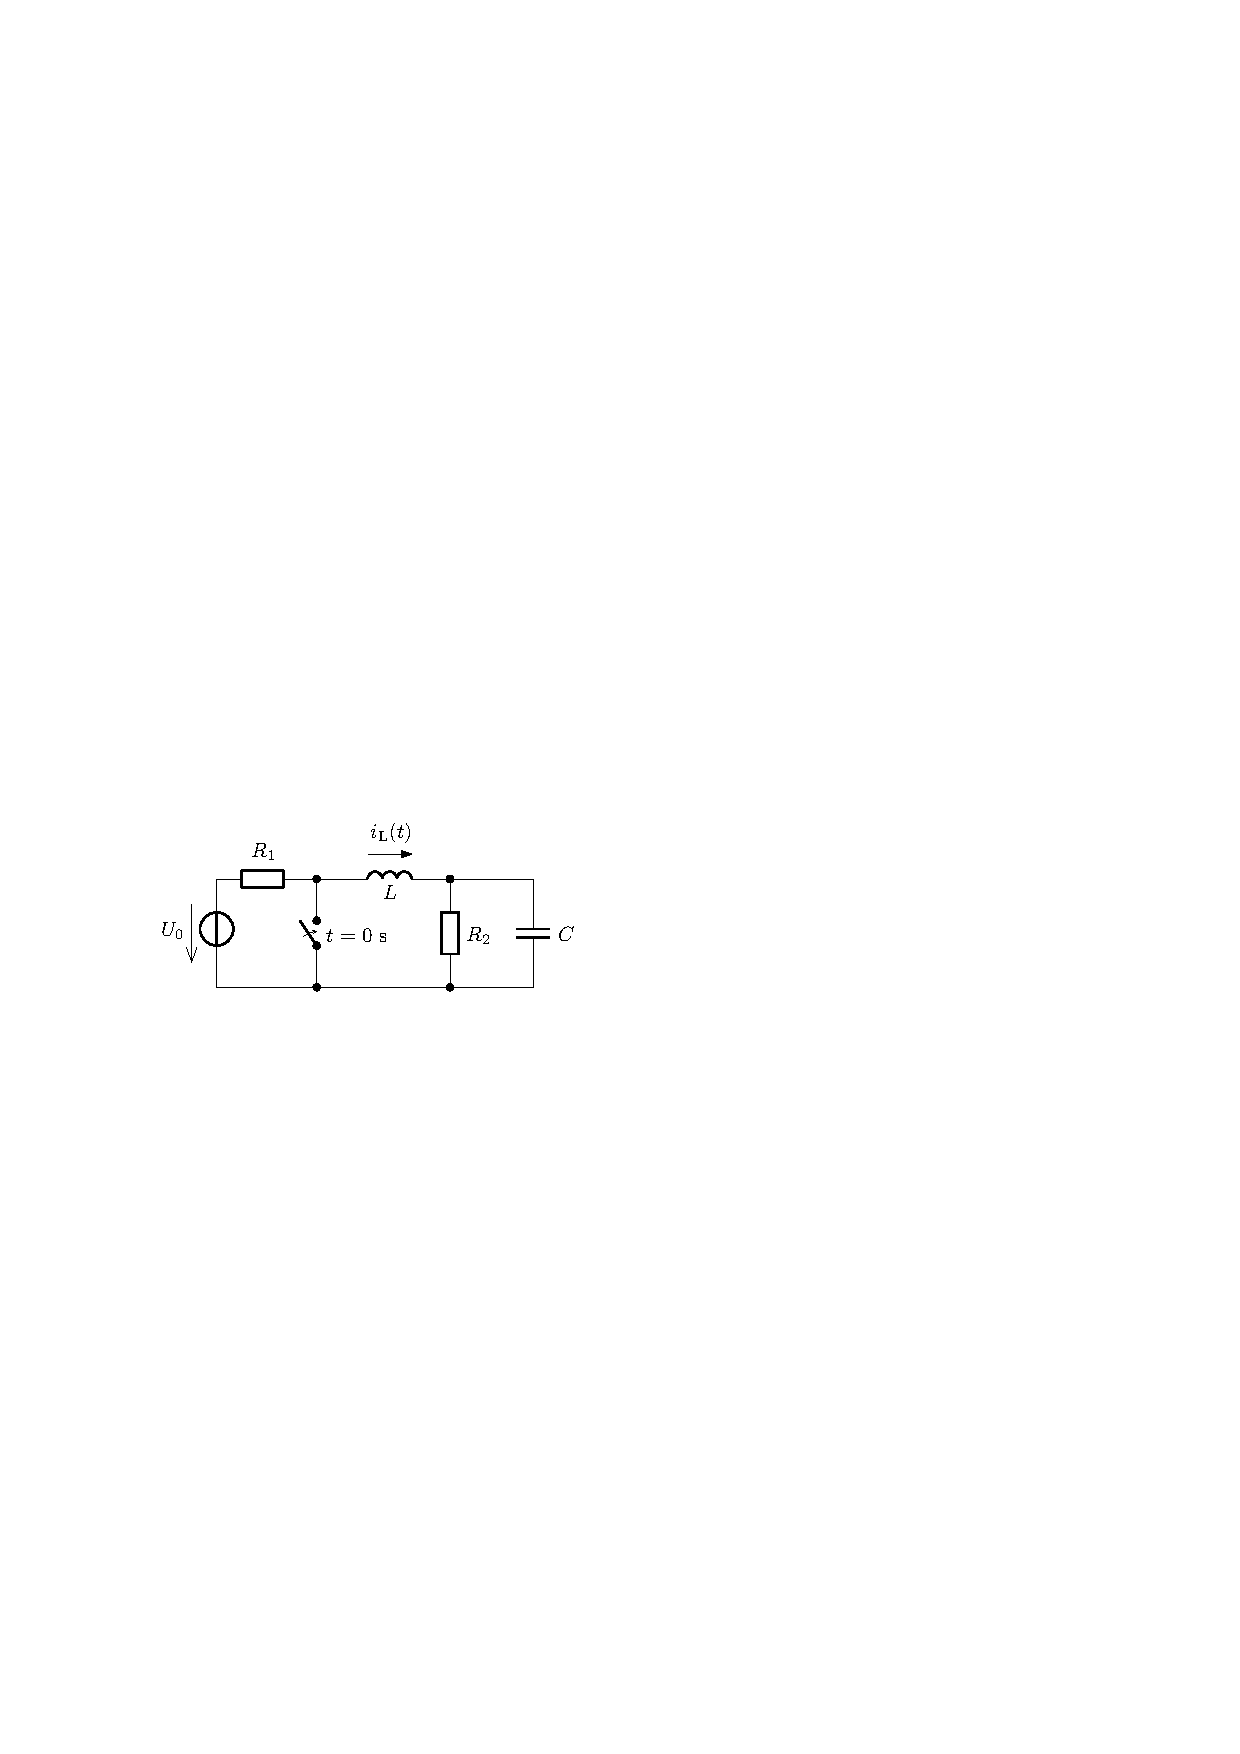
\includegraphics[]{prechodne_jevy/druhy_rad/priklad_1.pdf}
\caption{Obvod druhého řádu}
\label{fig:druhy_rad_priklad_1}
\end{figure}
